\documentclass[letterpaper,12pt]{article}

\usepackage[margin=1.0in]{geometry}
\usepackage{multirow}
\usepackage{tikz}
\usepackage{amsmath}
\usepackage{hyperref}
\usepackage{standalone}

\usetikzlibrary{shapes.geometric, arrows, fit}

\setlength\parindent{0pt}

\newcommand{\specialcell}[2][c]{\begin{tabular}[#1]{@{}c@{}}#2\end{tabular}}
\newcommand{\xxx}[1]{{\color{red}\bf #1}}
\newcommand{\AxisRotator}[1][rotate=0]{\tikz [x=0.25cm,y=0.60cm,line width=.2ex,-stealth,#1] \draw (0,0) arc (-150:150:1 and 1);}

\begin{document}

\title{\textbf{T-Shirt Cannon Robot User Guide}}
\author{Hazen Eckert \hspace{3mm} Omar Hasan \hspace{3mm} Ryan Marcotte \hspace{3mm} Ridhwaan Rahman}
\date{\today}
\maketitle

\begin{center}
    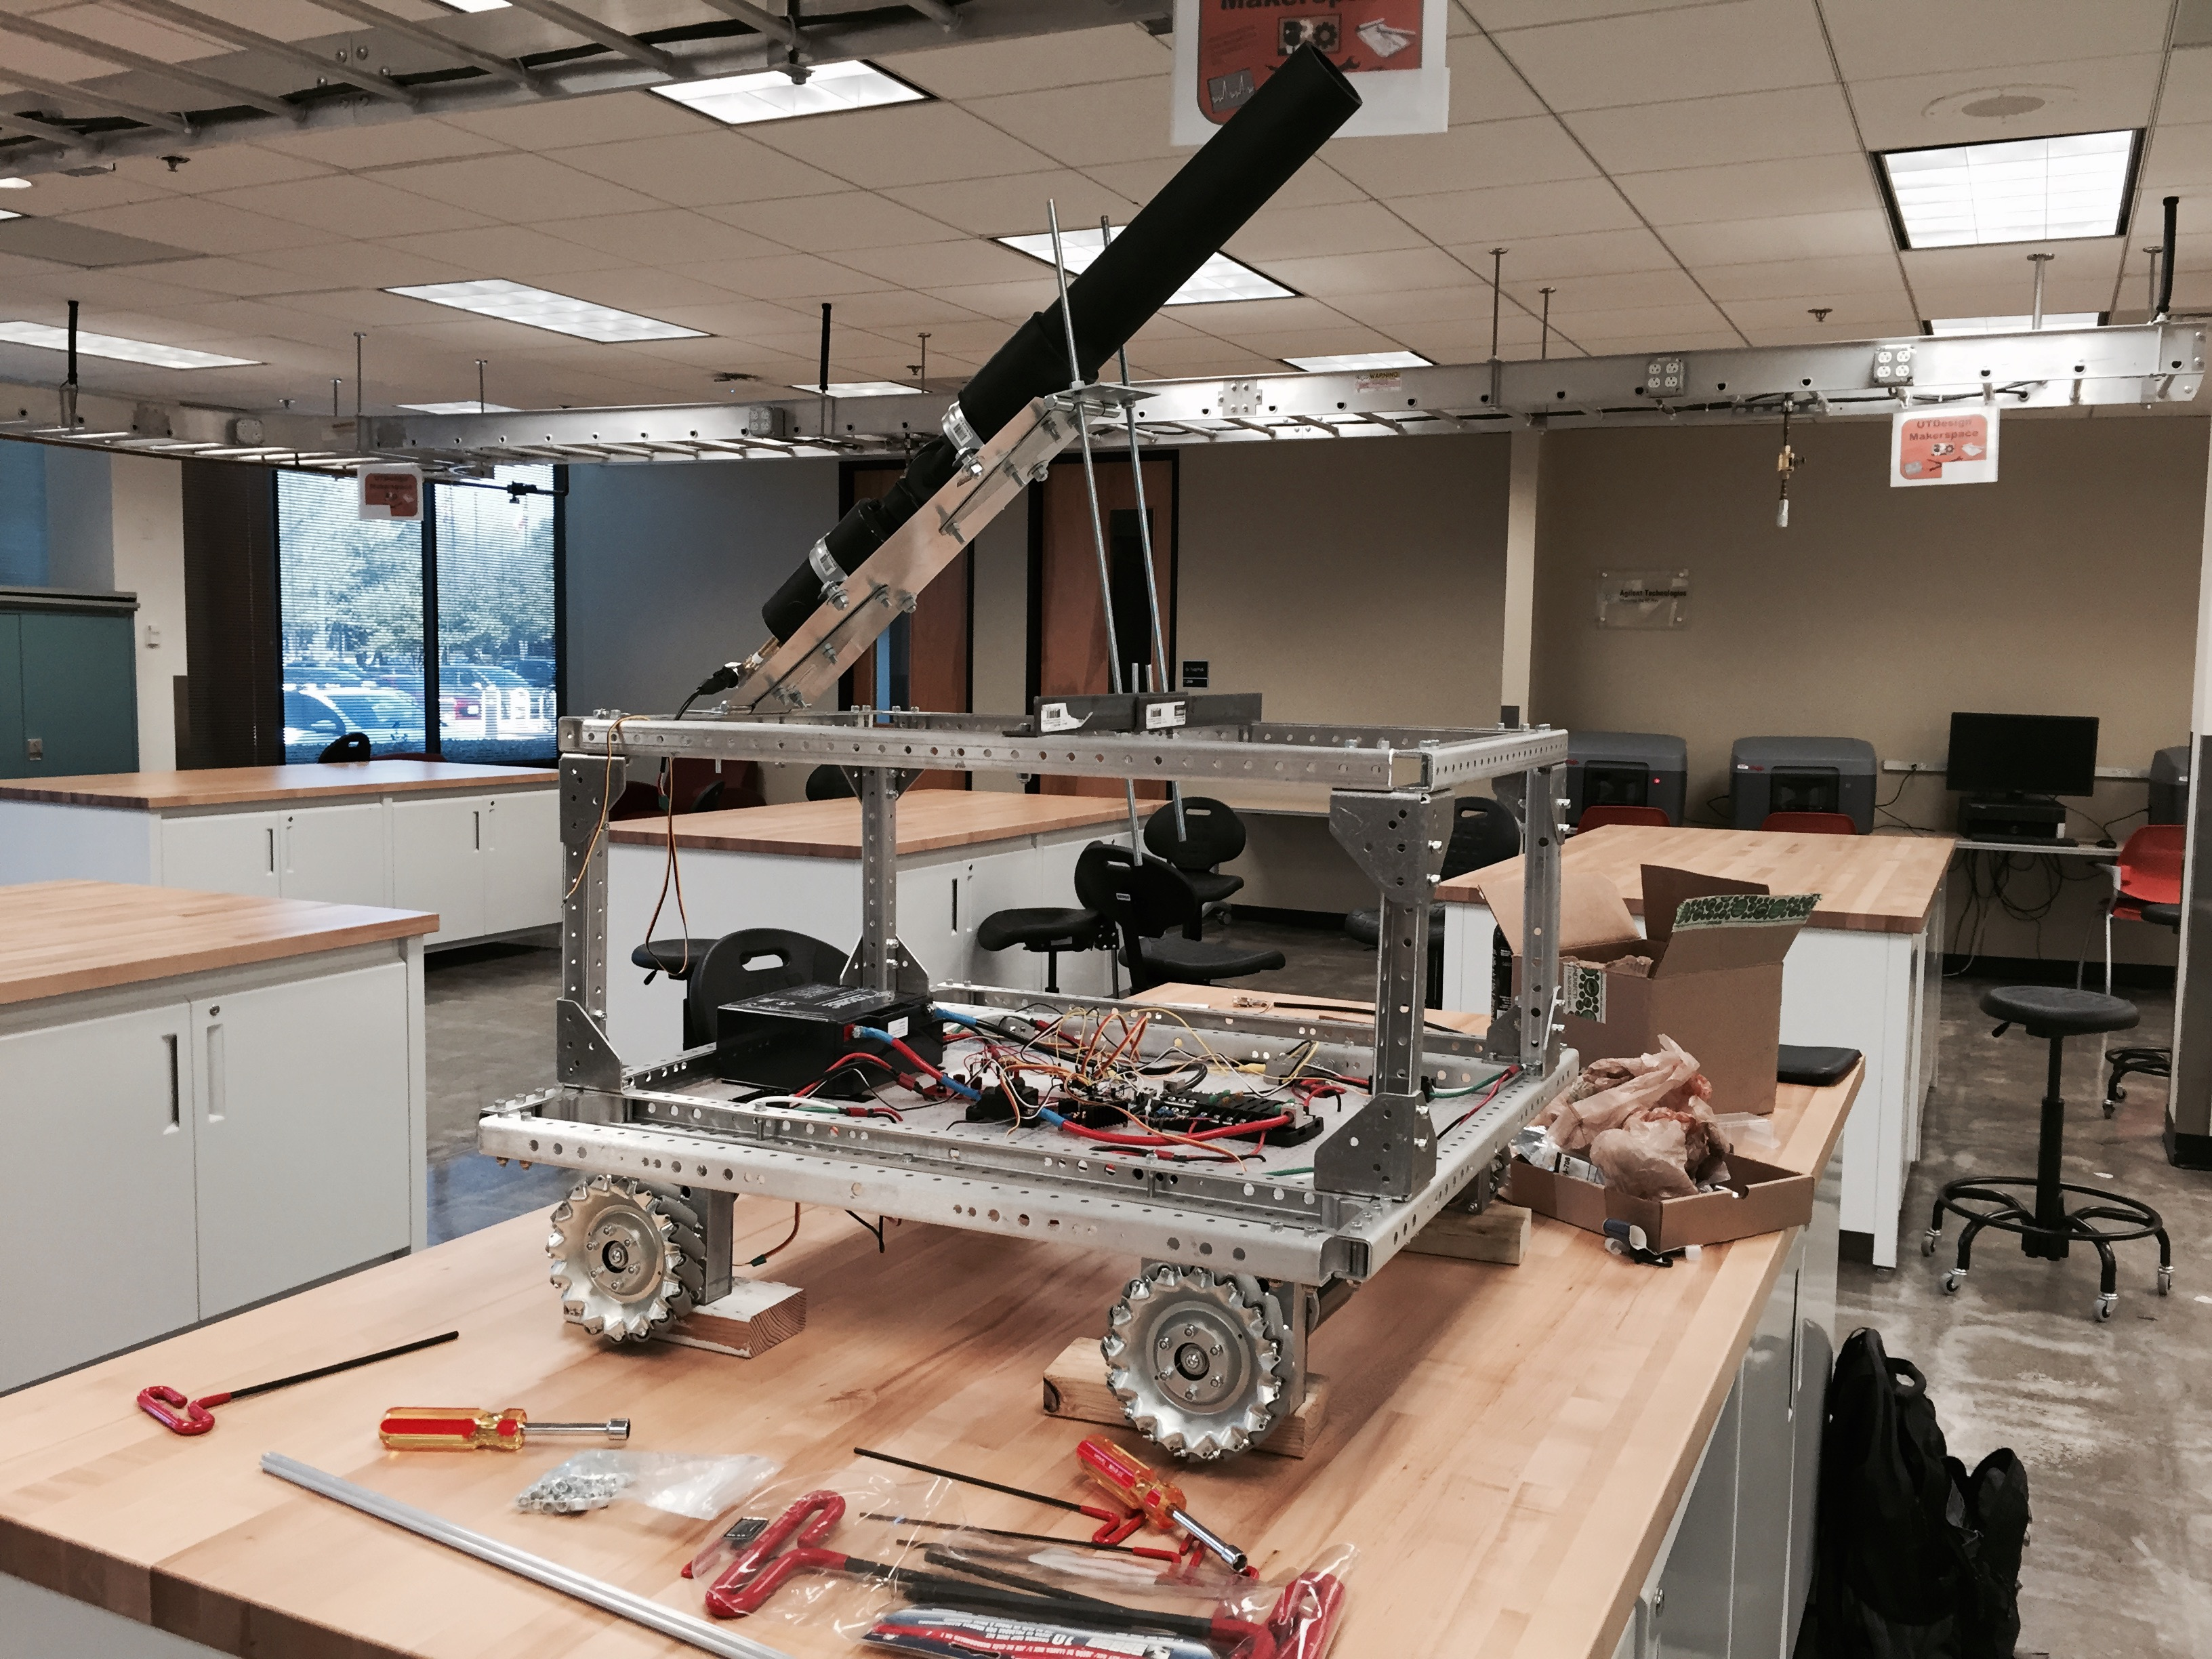
\includegraphics[width=15cm]{./pics/chassis/robot.jpg}
\end{center}

\pagebreak

\section*{Preface}
The purpose of this document is to both instruct the user on how to operate the
robot as well as inform them about its various quirks. At the time of this
document's writing, the repository that contains the source code for the
robot's processors as well as for the Java app that is used to control it
can be found here (\url{https://github.com/cometcannon/tshirt-cannon-robot}).
Should the link to the repo change, one might be able to find it by searching
github for an organization named "commetcannon".\\

If you find anything wrong with this document and you know LaTeX, feel free to
correct it. And finally, if you have any questions or concerns, feel free to
contact our mentor Dr. Nicholas Gans (ngans@utdallas.edu).\\

You can also try to contact one of the team members:\\
\begin{center}
\begin{tabular}{l l}
    Omar Hasan & omarhasan777@gmail.com \\
    Ridhwaan Rahman & ridhwaan.rahman99@gmail.com \\
    Ryan Marcotte & ryan@ryanjmarcotte.com \\
    Hazen Eckert & mr.mac.3.0.1@gmail.com \\
\end{tabular}
\end{center}
\addcontentsline{toc}{section}{Preface}

\pagebreak
\tableofcontents
\pagebreak

\section{Introduction}
\label{sec:intro}

\subsection{Purpose}
\label{sec:purpose}

\subsection{Problem Statement and Design Objectives}
\label{sec:probstatement}

\subsection{Design Process Summary}
\label{sec:designprocesssummary}

\subsection{Final Results Summary}
\label{sec:resultssummary}

\section{Review of Conceptual and Preliminary Design}
\label{sec:conceptualpreliminarydesign}

\subsection{Problem Analysis}
\label{sec:probanalysis}

\xxx{Review of problem}\\
\xxx{Summary of specifications}\\
\xxx{Discussion of main features of the design problem}\\
\xxx{Summary of basic engineering or technical approach}

\subsection{Decision Analysis}
\label{sec:decisionanalysis}

\xxx{Description of solution alternatives for the problem}\\
\xxx{Definition of effectiveness criteria}\\
\xxx{Discussion of decision analysis and final decision}

\section{Basic Solution Description}
\label{sec:basicsoldesc}

\xxx{Schematics and flow sheets defining all system components and their relationships}\\
\xxx{Analysis/balance of key parameters (voltage, current, power, timing or computing requirements, mechanical parameters, etc.)}\\
\xxx{Component sizing and component-level specifications}\\
\xxx{Initial system performance estimates}
\begin{figure}[h!]
  \centering

  \tikzstyle{block} = [rectangle, ultra thick, rounded corners, minimum width=3cm, minimum height=2cm,text centered, draw=black]
\tikzstyle{container} = [draw, ultra thick, rectangle, rounded corners, dashed, text width=11em, inner sep=3.5em]
  \tikzstyle{arrow} = [thick, ->, ultra thick, >=latex]
  \begin{tikzpicture}[node distance=2cm]
    \node (input) [align=center, xshift=-1cm] {\textbf{User}\\\textbf{Inputs}};
    \node (output) [right of=input, align=center] {\textbf{Video}\\\textbf{Display}};
    \node (app) [block, yshift=-2cm] {\textbf{Java App}};
    \node (ar9331) [block, right of=app, xshift=6cm, align=center] {\textbf{Atheros AR9331}};
    \node (atmega) [block, below of=ar9331, yshift=-2cm, align=center] {\textbf{ATmega32u4}};
    \node (rpi) [block, below of=app, left of=atmega, xshift=-6cm, yshift=2cm] {\textbf{Raspberry Pi}};

    \node (yun) [container, fit=(atmega) (ar9331)] {};
    \node (yun_text) [yshift=-0.3cm] at (yun.north) {\textbf{Yun}};

    \draw [arrow] (app.350) -- node[anchor=south, align=center, xshift=-7mm, yshift=-11mm] {\textbf{Velocity}\\\textbf{Commands}} (ar9331.190);
    \draw [arrow] (ar9331.170) -- node[anchor=north, align=center, xshift=-7mm, yshift=12mm] {\textbf{Status}\\\textbf{Updates}} (app.10);
    \draw [arrow] (ar9331.250) -- node[anchor=east, align=center] {\textbf{GPIO}\\\textbf{Commands}} (atmega.110);
    \draw [arrow] (atmega.70) -- node[anchor=west, align=center] {\textbf{Sensor}\\\textbf{Readings}} (ar9331.290);
    \draw [arrow] (rpi.70) -- node[anchor=east, align=center, xshift=2cm] {\textbf{Video}\\\textbf{Stream}} (app.290);
    \draw [arrow] (app.250) -- node[anchor=west, align=center, xshift=-2.7cm] {\textbf{Video}\\\textbf{Commands}} (rpi.110);
    \draw [arrow] (input) -- (app.134);
    \draw [arrow] (app.46) -- (output);
  \end{tikzpicture}
  \caption{Software System Diagram}
  \label{fig:system_diagram}
\end{figure}

\begin{figure}[h!]
  \centering
  \tikzstyle{block} = [rectangle, ultra thick, rounded corners, minimum width=2cm, minimum height=1cm,text centered, draw=black]
  \tikzstyle{dcvolt} = [solid, ultra thick, red];
  \tikzstyle{signal} = [solid, ultra thick, ->, >=stealth];

  \begin{tikzpicture}
    draw[help lines] (-6, -12) grid (12,1);
    \node (circuitbreaker) [block, align=center] {\textbf{Circuit}\\\textbf{Breaker}};
    \node (boost) [block, align=center, below of=circuitbreaker, xshift=-4cm, yshift=-2cm] {\textbf{Boost}\\\textbf{Converter}};
    \node (buck) [block, align=center, right of=boost, xshift=7cm] {\textbf{Buck}\\\textbf{Converter}};
    \node (mcu) [block, below of=buck, yshift=-1.25cm] {\textbf{MCU}};
    \node (triggersolenoid) [block, align=center, below of=boost, yshift=-3.5cm, xshift=-1.5cm] {\textbf{Trigger}\\\textbf{Solenoid}};
    \node (pressuresolenoid) [block, align=center, right of=triggersolenoid, xshift=2cm] {\textbf{Pressure}\\\textbf{Solenoid}};
    \node (encoders) [block, right of=pressuresolenoid, xshift=2cm] {\textbf{Encoders}};
    \node (pressuresensor) [block, align=center, right of=encoders, xshift=2cm] {\textbf{Pressure}\\\textbf{Sensor}};
    \node (camera) [block, align=center, right of=pressuresensor, xshift=2cm] {\textbf{Camera}\\\textbf{Module}};
    \node (esc) [block, right of=camera, xshift=2cm] {\textbf{ESC}};
    \node (motors) [block, below of=esc, xshift=-4.5cm, yshift=-1cm] {\textbf{Motors}};

    \draw [dcvolt] (circuitbreaker.north) -- +(0,0.5) node[anchor=south] {\textbf{+12V}};
    \draw [dcvolt] (circuitbreaker.south) -- +(0,-0.9) node[anchor=west, yshift=0.5cm] {\textbf{+12V}};
    \draw [dcvolt] (boost.north) -- +(0,1) -| +(4,1) node {};
    \draw [dcvolt] (buck.north) -- +(0,1) -| +(-4,1) node {};
    \draw [dcvolt] (esc.north) -- +(0,5.55) -| +(-5.5,5.55) node {};
    \draw [dcvolt] (buck.south) -- node[anchor=west, yshift=0.2cm] {\textbf{+5V}} (mcu.north);
    \draw [dcvolt] (encoders.north) -- +(0,2.7) -| +(3.5,2.7) node {};
    \draw [dcvolt] (pressuresensor.north) -- +(0,0.2) -| +(-3,0.2) node {};
    \draw [dcvolt] (camera.north) -- +(0,2.65) -| +(-2.5,2.65) node{};
    \draw [dcvolt] (boost.south) -- +(0,-1) node[anchor=west, yshift=0.5cm] {\textbf{+24V}};
    \draw [dcvolt] (triggersolenoid.north) -- +(0,2.4) -| +(1.5,2.4) node {};
    \draw [dcvolt] (pressuresolenoid.north) -- +(0,2.4) -| +(-1.5,2.4) node {};
    \draw [signal] (pressuresensor.east) -- +(0.5,0) -| +(0.5,0.75) -| +(-0.31, 0.75) -- (mcu.295);
    \draw [signal] (mcu.320) -- +(0,-0.8) -| +(3.5,-0.8) -| +(3.5,-1.75) -- (esc.west);
    \draw [signal] (encoders.east) -- +(0.5,0) -| +(0.5,0.95) -| +(2.39,0.95) -- (mcu.south);
    \draw [signal] (mcu.240) -- +(0,-0.6) -| +(-4.8,-0.6) -| +(-4.8,-1.75) -- (pressuresolenoid.east);
    \draw [signal] (mcu.220) -- +(0,-0.4) -| +(-7.4,-0.4) -| +(-7.4,-1.75) -- (triggersolenoid.east);
    \draw [signal] (esc.south) -- +(0,-1.5) -- (motors.east);
    \draw [signal] (motors.west) -- +(-3.5,0) -| (encoders.south);
  \end{tikzpicture}
  \caption{Electrical System Diagram}
  \label{fig:e_system}
\end{figure}

\section{Performance Optimization and Design of System Components}
\label{sec:optimization}
\xxx{Description of components and their component-level specifications} \\
\xxx{Design criteria used} \\
\xxx{Discussion of the technical approach used} \\
\xxx{Discussion of design details} \\
\xxx{Presentation and discussion of engineering drawings and schematics} \\
\xxx{Fabrication, construction, or production instructions and specifications} \\
\xxx{This section should provide any and all information necessary to ``build'' the component of the design you have focused on, all the way down to the number of nuts, bolts, transistors, wiring harness pin-outs, etc.} \\
\xxx{Summary of the final design results} \\
\xxx{Performance evaluation}

In order to command a desired robot velocity,
\begin{math}
  v=
  \begin{bmatrix}
    v_x \\
    v_y \\
    \omega_z
  \end{bmatrix}
\end{math}
, we calculate the wheel velocities as shown in Equations \ref{eq:rw_to_v}-\ref{eq:v_wheel_4}, according to Figure \ref{fig:robot_top_view}.

\begin{figure}[h!]
  \centering
  \includestandalone[width=\textwidth]{./tikz-figures/kinematics}
  \caption{Top View of Robot}
  \label{fig:robot_top_view}
\end{figure}

\begin{equation}
  v_{wheel}=r_{wheel}\omega_{wheel}
  \label{eq:rw_to_v}
\end{equation}
\begin{equation}
  v_{wheel\,0}=v_x-v_y-(l_1+l_2)\omega_z
  \label{eq:v_wheel_1}
\end{equation}
\begin{equation}
  v_{wheel\,1}=v_x+v_y+(l_1+l_2)\omega_z
  \label{eq:v_wheel_2}
\end{equation}
\begin{equation}
  v_{wheel\,2}=v_x-v_y+(l_1+l_2)\omega_z
  \label{eq:v_wheel_3}
\end{equation}
\begin{equation}
  v_{wheel\,3}=v_x+v_y-(l_1+l_2)\omega_z
  \label{eq:v_wheel_4}
\end{equation}

\begin{table}[h!]
  \centering
  \begin{tabular}{| c | c |}
    \hline
    \textbf{Motor} & \textbf{Position} \\
    \hline
    0 & Forward Left \\
    \hline
    1 & Forward Right \\
    \hline
    2 & Rear Right \\
    \hline
    3 & Rear Left \\
    \hline
  \end{tabular}
  \caption{Motor Numbers}
  \label{tab:motor_nums}
\end{table}

\section{Project Implementation, Operation, and Assessment}
\label{sec:implopassess}
\xxx{Details of implementation} \\
\xxx{Operational test results} \\
\xxx{Evaluation of results relative to design criteria (how well did it do?)} \\
\xxx{What changes are suggested by design results}

\section{Final Scope of Work Statement}
\label{sec:finalscope}
\xxx{Summarize what has been done} \\
\xxx{Summarize what still needs to be done} \\
\xxx{Lessons learned and suggestions for future activities} \\
\xxx{Describe any special details of the design that only you would know} \\
\xxx{Related project management issues} \\
\xxx{Address complete system life-cycle issues (marketing, sales, service, retirement)}

\section{Cost Estimation}
\label{sec:cost}
\xxx{Estimate of system cost (materials and construction)} \\
\xxx{Estimate of design cost (man-hours, materials and supplies, travel)} \\
\xxx{Other (such as construction or production or operating costs)}

\section{Project Management Summary}
\label{sec:projman}

\xxx{Tasks: what has been done} \\
\xxx{Tasks: what still needs to be done} \\
\xxx{Time: Gantt chart showing activities and their duration and order} \\
\xxx{Facilities} \\
\xxx{Personnel: summarize personnel needs to complete design; include a WBS}

\section{Conclusion}
\label{sec:conclusion}

\xxx{Restate purpose of report} \\
\xxx{Restate objectives} \\
\xxx{Summarize final design selection} \\
\xxx{Give costs and timeline} \\
\xxx{State willingness to ``keep the customer satisfied''}

\section{System Design Overview}

\section{Mechanical Components}
\subsection{Chassis}
\begin{center}
    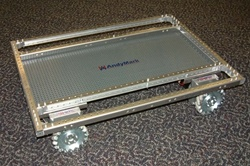
\includegraphics[width=11cm]{pics/chassis/andymark_chassis.jpg}
\end{center}

The Robot's Chassis is the AndyMark C-Chassis with Mecanum Wheel Drive. This
chassis was chosen among others because of its price, modularity, and size.

\subsubsection{Assembly}
\subsubsection{References}

\begin{table}[h!]
  \begin{tabular}{| c | c |}
    \hline
    \textbf{AndyMark Frame Assembly} &  http://files.andymark.com/am-0952AssemblyInstructions.pdf\\
    \hline
    \textbf{AndyMark Gearbox Assembly} &  http://files.andymark.com/x2010-toughbox-user-guide.pdf\\
    \hline
  \end{tabular}
  \label{tab:fire_cmd_msg}
\end{table}

\subsection{T-Shirt Cannon}
\begin{center}
    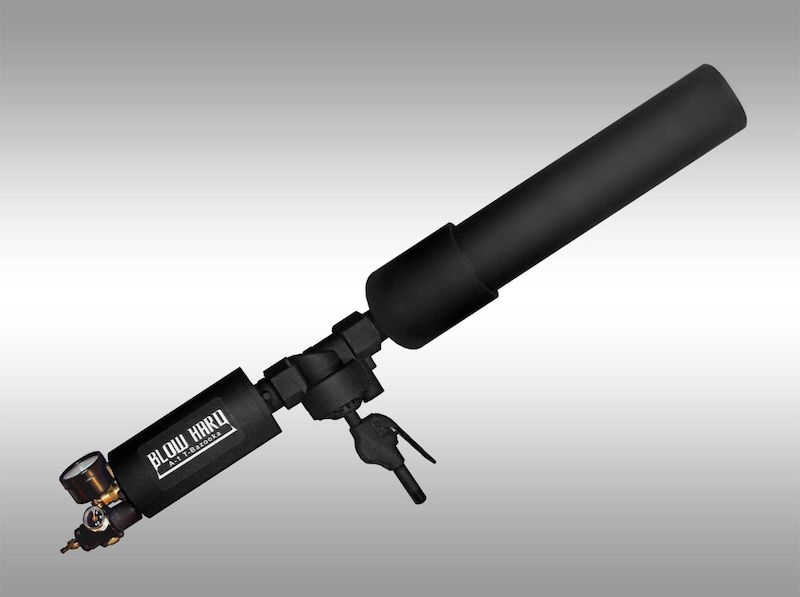
\includegraphics[width=11cm]{pics/cannon/blowhard_cannon.jpg}
\end{center}

\section{Electrical Components}

\subsection{Microcontrollers}
\subsubsection{AR9331}

\subsubsection{Serial Communication}
\label{sec:ar9331_serial_com}
The AR9331 and ATMega32U4 communicate via serial. To do this, we open the proper
serial device (\texttt{/dev/ttyATH0}) and use the straightforward
\texttt{write()} command. No further configuration of the serial device is
necessary.

\subsubsection{ATmega32u4}

\paragraph{Serial Communication}
\label{sec:atmega_serial_com}

Serial communication can occur between the ATmega and AR9331 chips or between
the ATmega chip and a computer connected via USB. In the former case, we read
and write to \texttt{Serial1}, whereas in the latter, we utilize the typical
\texttt{Serial}.


\subsubsection{Raspberry Pi}

\section{Software Components}
\subsection{Java Application}

\subsection{Network Protocols}

\subsubsection{Message Formats}

\paragraph{Computer to Robot}
\label{sec:comp_robot_msg}

\begin{table}[h!]
  \centering
  \begin{tabular}{| l | c | c | c | c | c | c | c | c |}
    \hline
    & 0 & 1 & 2 & 3 & 4 & 5 & 6 & 7 \\
    \hline
    \textbf{Kill Robot} & 0x47 & 0x41 & 0x4e & 0x53 & 0 & & & \\
    \hline
    \textbf{Kill Motors} & 0x47 & 0x41 & 0x4e & 0x53 & 1 & & & \\
    \hline
    \textbf{Command Horn} & 0x47 & 0x41 & 0x4e & 0x53 & 2 & & & \\
    \hline
    \multirow{2}{*}{\textbf{Command Velocity}} & \multirow{2}{*}{0x47} &\multirow{2}{*}{0x41} & \multirow{2}{*}{0x4e} &   \multirow{2}{*}{0x53} & \multirow{2}{*}{3} & v$_x$ & v$_y$ & $\omega_z$ \\
    & & & & & & -128 to 127 & -128 to 127 & -128 to 127 \\
    \hline
    \textbf{Query Motors} & 0x47 & 0x41 & 0x4e & 0x53 & 4 & & & \\
    \hline
    \textbf{Fire Cannon} & 0x47 & 0x41 & 0x4e & 0x53 & 5 & & & \\
    \hline
    \multirow{2}{*}{\textbf{Command Motor}} & \multirow{2}{*}{0x47} &\multirow{2}{*}{0x41} & \multirow{2}{*}{0x4e} &   \multirow{2}{*}{0x53} & \multirow{2}{*}{6} & Motor & Value & \\
    & & & & & & 0 to 3 & -128 to 127 & \\
    \hline
    \multirow{2}{*}{\specialcell{\textbf{Command and}\\\textbf{Control Velocity}}} & \multirow{2}{*}{0x47} &\multirow{2}{*}{0x41} & \multirow{2}{*}{0x4e} &   \multirow{2}{*}{0x53} & \multirow{2}{*}{7} & v$_x$ & v$_y$ & $\omega_z$ \\
    & & & & & & -128 to 127 & -128 to 127 & -128 to 127 \\
    \hline
    \textbf{Increase Pressure} & 0x47 & 0x41 & 0x4e & 0x53 & 8 & & & \\
    \hline
    \textbf{Query Pressure} & 0x47 & 0x41 & 0x4e & 0x53 & 9 & & & \\
    \hline
    \textbf{AVR Debug} & 0x47 & 0x41 & 0x4e & 0x53 & 10 & & & \\
    \hline
    \textbf{Atheros Debug} & 0x47 & 0x41 & 0x4e & 0x53 & 11 & & & \\
    \hline
  \end{tabular}
  \caption{Computer-to-Robot Message Specifications}
  \label{tab:comptorobotmsgspecs}
\end{table}

\paragraph{AR9331 to ATmega32u4}
\label{sec:ath_mega_msg}

\xxx{Query commands will start at 101, but we have yet to come up with the types that we need}

\begin{table}[h!]
  \centering
  \begin{tabular}{| c | c | c|}
    \hline
    \textbf{Byte} & 0-3 & 4 \\
    \hline
    \textbf{Description} & \specialcell{Magic\\Bytes} & \specialcell{Command\\Type} \\
    \hline
    \textbf{Value} & 0x47414e53 & 0 \\
    \hline
  \end{tabular}
  \caption{Kill Command Message Format}
  \label{tab:ath_kill_cmd_msg}
\end{table}

\begin{table}[h!]
  \centering
  \begin{tabular}{| c | c | c|}
    \hline
    \textbf{Byte} & 0-3 & 4 \\
    \hline
    \textbf{Description} & \specialcell{Magic\\Bytes} & \specialcell{Command\\Type} \\
    \hline
    \textbf{Value} & 0x47414e53 & 1 \\
    \hline
  \end{tabular}
  \caption{Keep Alive Command Message Format}
  \label{tab:ath_keep_alive_cmd_msg}
\end{table}

\begin{table}[h!]
  \centering
  \begin{tabular}{| c | c | c | c | c |}
    \hline
    \textbf{Byte} & 0-3 & 4 & 5 & 6 \\
    \hline
    \textbf{Description} & \specialcell{Magic\\Bytes} & \specialcell{Command\\Type} & \specialcell{Motor\\Number} & Value \\
    \hline
    \textbf{Value} & 0x47414e53 & 2 & 0-3 & -128 to 127 \\
    \hline
  \end{tabular}
  \caption{Individual Motor Command Message Format}
  \label{tab:ath_ind_motor_cmd_msg}
\end{table}

\begin{table}[h!]
  \centering
  \begin{tabular}{| c | c | c | c | c | c | c |}
    \hline
    \textbf{Byte} & 0-3 & 4 & 5 & 6 & 7 & 8\\
    \hline
    \textbf{Description} & \specialcell{Magic\\Bytes} & \specialcell{Command\\Type} & \specialcell{Motor 0\\Value} & \specialcell{Motor 1\\Value} & \specialcell{Motor 2\\Value} & \specialcell{Motor 3\\Value} \\
    \hline
    \textbf{Value} & 0x47414e53 & 3 & -128 to 127 & -128 to 127 & -128 to 127 & -128 to 127 \\
    \hline
  \end{tabular}
  \caption{All Motor Command Message Format}
  \label{tab:ath_all_motor_cmd_msg}
\end{table}

\begin{table}[h!]
  \centering
  \begin{tabular}{| c | c | c | c | c |}
    \hline
    \textbf{Byte} & 0-3 & 4 & 5 \\
    \hline
    \textbf{Description} & \specialcell{Magic\\Bytes} & \specialcell{Command\\Type} & \specialcell{Motor\\Number} \\
    \hline
    \textbf{Value} & 0x47414e53 & 4 & 0-3 \\
    \hline
  \end{tabular}
  \caption{Individual Motor Command for Returning Measured Angular Velocity}
  \label{tab:ath_ind_motor_cmd_msg}
\end{table}

\begin{table}[h!]
  \centering
  \begin{tabular}{| c | c | c |}
    \hline
    \textbf{Byte} & 0-3 & 4 \\
    \hline
    \textbf{Description} & \specialcell{Magic\\Bytes} & \specialcell{Command\\Type} \\
    \hline
    \textbf{Value} & 0x47414e53 & 5 \\
    \hline
  \end{tabular}
  \caption{Fire Command Message Format}
  \label{tab:comp_fire_cmd_msg}
\end{table}

\begin{table}[h!]
  \centering
  \begin{tabular}{| c | c | c | c | c |}
    \hline
    \textbf{Byte} & 0-3 & 4 & 5 & 6 \\
    \hline
    \textbf{Description} & \specialcell{Magic\\Bytes} & \specialcell{Command\\Type} & \specialcell{Motor\\Number} & Value \\
    \hline
    \textbf{Value} & 0x47414e53 & 6 & 0-3 & -128 to 127 \\
    \hline
  \end{tabular}
  \caption{Individual Motor Velocity Command Message Format}
  \label{tab:ath_ind_motor_cmd_msg}
\end{table}

\begin{table}[h!]
  \centering
  \begin{tabular}{| c | c | c | c | c | c | c |}
    \hline
    \textbf{Byte} & 0-3 & 4 & 5 & 6 & 7 & 8\\
    \hline
    \textbf{Description} & \specialcell{Magic\\Bytes} & \specialcell{Command\\Type} & \specialcell{Motor 0\\Value} & \specialcell{Motor 1\\Value} & \specialcell{Motor 2\\Value} & \specialcell{Motor 3\\Value} \\
    \hline
    \textbf{Value} & 0x47414e53 & 7 & -128 to 127 & -128 to 127 & -128 to 127 & -128 to 127 \\
    \hline
  \end{tabular}
  \caption{All Motor Velocity Command Message Format}
  \label{tab:ath_all_motor_cmd_msg}
\end{table}

\begin{table}[h!]
  \centering
  \begin{tabular}{| c | c | c | c | c | c |}
    \hline
    \textbf{Byte} & 0-3 & 4 & 5-6 \\
    \hline
    \textbf{Description} & \specialcell{Magic\\Bytes} & \specialcell{Command\\Type} & \specialcell{Pressure\\(Big Endian)} \\
    \hline
    \textbf{Value} & 0x47414e53 & 8 & 0-1023 \\
    \hline
  \end{tabular}
  \caption{Set Pressure Regulation Command}
  \label{tab:ath_ind_motor_cmd_msg}
\end{table}
\paragraph{ATmega32u4 to AR9331}
\label{sec:mega_ath_msg}

\section{Operating the Robot}

\subsection{Running the video stream from outside the app}
nc 192.168.1.1 5001 | mplayer -fps 60 -cache 1024 -

\section{Troubleshooting}

\subsection{Mechanical Issues}
\subsubsection{Chassis}
\subsubsection{T-Shirt Cannon}

\begin{center}
    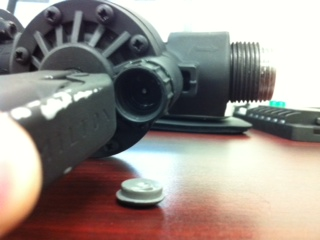
\includegraphics[width=11cm]{pics/cannon/broken_release_valve.jpg}
\end{center}

\subsection{Electrical Issues}

\subsection{Software Issues}
\subsubsection{Site to install xbox controller drivers}
OSX: http://tattiebogle.net/index.php/ProjectRoot/Xbox360Controller/OsxDriver


\end{document}
